\documentclass[a4paper]{book}
\usepackage{amsmath}
\usepackage{algorithm}
\usepackage[noend]{algpseudocode}
\usepackage{graphicx}
\usepackage[numbers,sort]{natbib}
\usepackage{array}
\usepackage{amssymb}
\usepackage{tabularx}
\usepackage{wrapfig}
\usepackage{subcaption}
\usepackage[numbers,sort]{natbib}
\usepackage{geometry} 	
\let\oldemptyset\emptyset
\let\emptyset\varnothing

\graphicspath{ {Figures/}}

\usepackage{listings}
\usepackage{xcolor}
\lstdefinestyle{customc}{
  belowcaptionskip=1\baselineskip,
  breaklines=true,
  frame=L,
  xleftmargin=\parindent,
  language=C,
  showstringspaces=false,
  basicstyle=\footnotesize\ttfamily,
  keywordstyle=\bfseries\color{green!40!black},
  commentstyle=\itshape\color{purple!40!black},
  identifierstyle=\color{blue},
  stringstyle=\color{orange},
}

\lstdefinestyle{customasm}{
  belowcaptionskip=1\baselineskip,
  frame=L,
  xleftmargin=\parindent,
  language=[x86masm]Assembler,
  basicstyle=\footnotesize\ttfamily,
  commentstyle=\itshape\color{purple!40!black},
}


\lstset{escapechar=@,style=customc}

\geometry{b5paper}


%\usepackage{todonotes}
% Title Page
\title{SPECCY - check it out}
\author{Julian Ho-yin Lam}


\begin{document}
%\maketitle
%This is the Titlepage
%%=========================================
\thispagestyle{empty}

\includegraphics[scale=0.3]{Figures/ntnu}
\mbox{}\\[6pc]
\begin{center}
\Large{TDT4900  Computer Science, Master's Thesis}\\[1pc]
\Huge{Optimization of Seed Selection for Information Diffusion with High Level Synthesis}\\[2pc]

\Large{Julian Lam}\\[1pc]
\large{Spring 2016}\\[2pc]


Department of Computer and Information Science\\
Norwegian University of Science and Technology
\end{center}
\vfill

\noindent Supervisor 1: Donn Alexander Morrison

\noindent Supervisor 2: Yaman Umuroglu
\setcounter{page}{0}
\pagenumbering{roman}
\section*{Abstract}

Information diffusion is where a message or data is passed from vertex to vertex in a network via edges. Information diffusion is often used for simulations in network research because it estimates how information propagates through a network. A set of vertices that in initial state contains the data is known as the \textit{seed nodes}. The diffusion starts at the seed nodes and propagates over the network. Finding the optimal seed nodes is a crucial part of information diffusion. The seed nodes are the optimal targets to start passing messages during a disaster scenario, vaccinate to prevent the spreading of a disease or even targets for viral marketing. Finding these seed nodes is an NP-hard problem and require a significant amount of computation. One common used model in information diffusion is the \textit{independent cascade model} (ICM). ICM can be performed as a \textit{sparse matrix-vector multiplication} (SPMV). 
\chapter*{Sammendrag}
Information diffusion er n\r{a}r en melding eller data blir sendt fra node til node via kantene i et nettverk. Information diffusion er ofte brukt i simulering i nettverks forskning siden den kan estimere hvordan data propagerer gjennom et nettverk. Et sett med noder som starter med dataen er kjent som \textit{seed nodes}. Diffusjonen starter ved \textit{seed nodes} og propagerer gjennom hele nettverket. \r{a} finne de mest optimale \textit{seed nodes} er en essensiell del av \textit{Information Diffusion}, siden de kan spre bedskjedet til mest mulig mennesker under en krisesituasjon, ved \r{a} vaksinere dem s\r{a} kan man forhindre spredning av sykdommer, eller s\r{a} er de \textit{seed node} de optimale kandidater for \r{a} promotere produkt.

\r{A} finne disse \textit{seed nodes} er et NP-hard problem og krever stor mengde beregninger. En vanlig brukt modell er kjent som Independent cascade model(ICM).  ICM kan bli gjort via \textit{sparse matrix-vector multiplication} (SPMV). Ved \r{a} bruke en applikasjons spesifikk hardware akselerator, sp kan vi optimalisere diffusjons prosessen og \textit{Seed selection}.  High level synthesis har i de siste f\r{a}tt mye mer oppmerksomhet. HLS  transformerer h{\o}y-niv\r{a} implementasjoner til lav-niv\r{a} design. Ved hjelp av HLS kan vi utvikler applikasjons spesifikk \textit{intelectual property core} (IP core) som vi implementerte i en \textit{field-programmable gate array} (FPGA) og utf{\o}re \textit{seed selection}

\section*{Assignment}
Information diffusion is a field of network research where a message, starting
at a set of seed nodes, is propagated through the edges in a graph according to
a simple model. Simulations are used to measure the coverage and speed of the
diffusion and are useful in modelling a variety of phenomena such as the spread
of disease, memes on the Internet, viral marketing and emergency messages in
disaster scenarios.

The effectiveness of a given spreading model is dependent on the initially
infected nodes, or seeds. Seed selection for an optimal spread is an NP hard
problem and is normally approximated by selecting high-degree nodes or using
heuristic methods such as discount-degree or choosing nodes at different levels
of the k-core.

High-level synthesis (HLS) is becoming an important tool in the
optimization/acceleration of algorithms in hardware. Starting with an algorithm
written in a high-level language such as C or C++, HLS aids with hardware
design by providing a methodology and tools that guide the developer through
the design process.

This project should employ HLS as a design methodology for hardware accelerated
seed selection in large graphs. The student will study seed selection for a
given diffusion model, write a high-level model, and use HLS to implement a
hardware design that exploits parallelism in the seed selection algorithm in
order to improve performance over a GPCPU implementation.

\tableofcontents
\listoffigures
\listoftables
\setcounter{page}{0}
\pagenumbering{arabic}
\chapter{Introduction} \label{intro}

\section{Motivation}
\textit{Information Diffusion} is a field in network research where a message, or data, is propagated through a \textit{network} or a \textit{graph}. The message originates from a chosen set of vertices, known as \textit{seed nodes}. These seed nodes pass the message to its neighbours through the edges and thus propagates the message over the network. The effectiveness of the diffusion is measured through the spread and the speed of propagation and is dependent on the chosen seed nodes. By finding the most optimal set of seed nodes, we can potentially stop an epidemic by vaccinating influential vertices, we can find important targets for viral marketing by giving free samples, and use this information to spread messages quickly during disaster scenarios\cite{InformationDiffusionThroughBlogspace} \cite{Romero:2011:DMI:1963405.1963503}.

There are multiple studies done regarding information diffusion, \cite{InformationDiffusionThroughBlogspace},\cite{cha2010measuring},  \cite{5694014},  \cite{InfoDiffAndExternalInfluInNetworks}. But as far as we know, there are none that focus on optimizing the seed selection in hardware. The current seed selection algorithm is a greedy solution\cite{greedyInfluenc2005}, where every set of vertices is tested and the set with the best coverage and time is chosen. This is a time-consuming process and highly parallelizable, which makes it a good candidate for \textit{Field-programmable gate arrays}(FPGAs). 

\textit{High Level Syntesis} (HLS) transform high level behaviour and constraints to lower level design.\cite{52214}. It makes it possible to implement an algorithm in high level language, C or C++, and generate an optimal design in \textit{verilog} or \textit{VHDL}. Verilog and VHDL are hardware descriptive languages designed to describe digital systems \cite{thomas2008verilog}. 

Unlike traditional hardware design, HLS allows designers with limited knowledge of hardware design to create an optimal custom \textit{Intellectual property core}(IP-core). In HLS, programmers can test out different optimization schemes in a short period of time, thus reducing development overhead.  

In this thesis, we have implemented a simple IP-core that performs information diffusion using the \textit{Independen Cascade model} (ICM) as \textit{Breadth-First Search} (BFS) over boolean semiring. This is done by using HLS as the development tool. 


\section{Assignment Interpretation}
From the assignment text, these task were chosen as the main focus of this thesis:\\ \hfil \\ \hfil
\textbf{Task 1 \textit{(mandatory)}} Implement Information Diffusion as Sparse matrix vector multiplication, with high level language C.  \\ \hfil \\ \hfil
\textbf{Task 2 \textit{(mandatory)}} Tailor the implementation of Information Diffusion for synthesise with Vivado HLS.   \\ \hfil \\ \hfil
\textbf{Task 3 \textit{(optional)}} Implement said design on a  Zynq FPGA board. \\ \hfil \\ \hfil
\textbf{Task 4 \textit{(optional)}} Extend the system to be able to handle graph in the size of toy graphs(containing $2^{26})$ vertices) \\ \hfil \\ \hfil


\section{Report Structure}
We have here the basic outline for this report and a short overview of the remainder of this report:\\ \hfill

\textbf{Chapter 2: Background} contains the theory regarding networks, information diffusion, matrix-vector multiplication and high level synthesis. \\ \hfil \\ \hfil
\textbf{Chapter 3: Related Work} gives a short introduction of the state of the art of HLS implementations, information diffusion research and different optimization of BFS.\\ \hfil \\ \hfil
\textbf{Chapter 4: Design and Implementation} present our implementation of our IP-core and give a brief introduction regarding HLS implementation and optimization.  \\ \hfil \\ \hfil
\textbf{Chapter 5: Result and Discussion} will compare the result our core generated compared to a C-simulation. We will also discuss some of the design choices regarding the IP-core. \\ \hfil \\ \hfil
\textbf{Chapter 6: Future Work} present how our design can be further improved. \\ \hfil \\ \hfil
\textbf{Chapter 7: Conclusion} provides concluding remarks regarding this paper and a summary of the identified tasks. \\ \hfil \\ \hfil
\chapter{Background} \label{background}

In this chapter, we will look at the fundamental concepts and theory of the different diffusion models, seed selection algorithms and perform BFS over the boolean semiring. We will also have a look at HLS and specifications of the Zedboard. This chapter will contain notations that we will use throughout the report.

 We will look at the independent cascade model, which is a special case of breadth first search  \cite{HybridBFS2015}. By looking at how to improve BFS, we can apply such optimization to ICM and the seed selection algorithm.
 \\
 

\section{Information Diffusion}
Information diffusion is looking at how information is propagated through a network. A vertex can be either activated(infected) or inactivated(healthy/noninfected), each vertex can spread the contagion(activation,infection) to their neighbour. Some examples would be how a meme, a trend or a disease is spread through a community. The process consists of a set of starter vertices, which we will call seed nodes, which are "infected" at initial time step. During each time step, there are a percentage $p_g$ where the "infected" vertices would "infect" its neighbours. Seed nodes is a set of $k$ vertices that in the initial time-step are infected. They will pass on the information/infection during each iteration, and the information/infection will propagate through the network. 

 
\section{Basic Diffusion Models}
For information diffusion, two common models are used for simulations. Those are the \textit{linear threshold model}(LTM) and the \textit{independent cascade model}(ICM) \cite{MaximizeSpread2003}.

ICM is a model where each spread of contagion is dependent on a "coin flip". Each person has a chance to be contaminated, and during each diffusion, dependent on the result of the coin flip, that person is either contaminated/infected or healthy. In ICM, an infected person can not reinfect the previously spared person. The probability of infection can be either globally, or locally. In Figure \ref{fig:ICM1}, we can see a situation where \textit{C} have five neighbour,\textit{A},\textit{B},\textit{D},\textit{E} and \textit{F}. In the initial state, only C is infected. Five separate "coin flips" was done and resulted in three more activations as shown in Figure \ref{fig:ICM2}. C spread the contagion to three other people, while A and F were spared. In Figure \ref{fig:ICM3} F is activated by E. 

%Fiks figur og tekst overfor.%
%Forlar hvordan ICM Funker%

\begin{figure}[!ht]
    \begin{subfigure}{0.3\textwidth}
        \includegraphics[width=\textwidth]{Figures/ICM_step1}
        \caption{Initial state} 
        \label{fig:ICM1}
    \end{subfigure}
    \begin{subfigure}{0.3\textwidth}
        \includegraphics[width=\textwidth]{Figures/ICM_step2}
        \caption{second state, activated by C is marked blue} 
        \label{fig:ICM2}
    \end{subfigure}
    \begin{subfigure}{0.3\textwidth}
        \includegraphics[width=\textwidth]{Figures/ICM_step3}
        \caption{third state, activated by E is marked red, no more activation from C} 
        \label{fig:ICM3}
    \end{subfigure}
    \caption{Independent cascade model}
    \label{fig:ICM_step}
\end{figure}


For the LTM activation is not dependent on a probability and a "coin flip", but an internal threshold of activated neighbours. The spread of contagion is dependent on how large of a fraction of their neighbour is activated. For our example, let say that for a person to be infected, 0.6 of their total neighbour must be infected before they can contract the contagion. In Figure \ref{fig:LTM}, we see that in the initial state \textit{A},\textit{B} and \textit{D} are infected. For \textit{C}, more than 0.6 of its total neighbours are activated, this resulted in an activation of it too as seen in Figure \ref{fig:linearThresh3}.  We can see that both \textit{E} and \textit{F} have only 0.5 of their neighbours activated, and thus in Figure \ref{fig:linearThresh3} no more activation is presence.


%FIX these figures theta_V is actually b_v%
\begin{figure}[!ht] \label{fig:LTM}
    \begin{subfigure}{0.3\textwidth}
        \includegraphics[width=\textwidth]{Figures/LTM_step1}
        \caption{Initial state, A,B,D is activated.} 
        \label{fig:linearThresh}
    \end{subfigure}
    \begin{subfigure}{0.3\textwidth}
        \includegraphics[width=\textwidth]{Figures/LTM_step2}
        \caption{Second state, S is activated and marked blue.} 
        \label{fig:linearThresh2}
    \end{subfigure}
    \begin{subfigure}{0.3\textwidth}
        \includegraphics[width=\textwidth]{Figures/LTM_step2}
        \caption{Third state, no more activation, since both E and F have less then 0.6 activated neighbours.} 
        \label{fig:linearThresh3}
    \end{subfigure}
    \caption{Linear Threshold mode}
\end{figure}


A real world example of the LTM would be e.g. A new product on the market. People would adopt the new product it enough of their acquaintance is using it (activated). While ICM would be more directed marketing. Where free samples are given to some users. Those users would then promote the product and potentially spread the product to other.

ICM is a special case of BFS, both algorithm traverse graphs in a level-by-level approach. The difference is that for ICM, each node is not guaranteed to be activated. If an ICM had an activation chance of a hundred percent, then the ICM would be the same as BFS.


\section{Breadth First Search}
BFS is a tree traversal algorithm. BFS starts at the root vertex \textit{$v_r$}. The algorithm then stores all $v_r$s children vertices in a \textit{queue}. The algorithm then takes the first vertex from the queue, \textit{$v_1$} and stores all the children vertices to \textit{$v_1$} in the back of the queue. This process continues until the queue is empty and all the vertices have been iterated over. 

BFS is a common graph iteration algorithm but is often limited by the irregular memory access where the algorithm has to find the data stored in different spaces in memory.

%%forklar hva frontier er for noe
\begin{algorithm}
\caption{Breadth First Search}
\begin{algorithmic}[1]
\State{$dist[\forall \textit{v} \in V] = -1; currentQ, nextQ = \oldemptyset$}
\State $step = 0; dist[root] = step$
\State ENQUEUE(nextQ,root)
\While {$nextQ\neq \oldemptyset $}
\State $currentQ = newxtQ; nextQ = \oldemptyset$
\State $step = step+1$
\While {$currentQ \neq \oldemptyset$}
\State$ u$ = DEQUEUE(currentQ)
\For {$v \in Adj[u]$}
\If {$dist[v] == -1 $}
\State $dist[v] = step$
\State ENQUEUE(nextQ, v)
\EndIf
\EndFor
\EndWhile
\EndWhile
\Return dist
\end{algorithmic}
\end{algorithm}


 
\subsection{BFS to Data Diffusion}

The motivation for transforming breadth first search as matrix-vector multiplication is that displaying the graph algorithm as a matrix multiplication can display the data access pattern for the algorithm and can be readily optimized  \cite{AlgoToMath}.

As mentioned before, ICM is a special case of the breadth first search. By modifying the algorithm proposed earlier, we can, in theory, perform ICM with matrix-vector multiplication.  

\section{Matrix Notations}
Networks can be represented as \textit{sparse adjacency matrices} \cite{AlgoToMath} \cite{McAndrew1963}. By representing networks as a sparse matrix, we can often discover different ways to optimize the algorithm, or a different structure to store the data. The adjacency matrix, in particular, is an interesting way to represent the graph. A graph $G =(V, E)$, G have N vertices and M edges, and this correspond to a N$\times$N adjacency matrix called A. If A(i,j)=1, then there is an edge from $v_i$ to $v_j$. Otherwise, it is 0. In Figure:\ref{fig:AdjacencyM}, we can see how a undirected graph can be represented as an adjacency matrix. Each square symbolises a connection between two vertices. To generate a undirected graph as an adjacency matrix, the matrix must be mirrored diagonally, meaning if A(i,j)=1, then A(j,i)=1, if this is not true, then the matrix would be representing a directed graph.

\subsection{Sparse Matrix}
A sparse matrix is a matrix containing few nonzero entries. A social graph with few edges would often be represented as a sparse matrix. Since sparse matrices only have few non-zero elements, by storing only the non-zero elements, we can have savings in memory. 

\begin{figure}[!ht]
    \begin{subfigure}{0.3\textwidth}
    \includegraphics[width=0.8\textwidth]{Figures/AdjacencyMatrix}
    \caption{The adjacency matrix}
    \label{fig:AdjacencyM}
    \end{subfigure}
    \begin{subfigure}{0.3\textwidth}
    \includegraphics[width=0.8\textwidth]{Figures/simpleGraph}
    \caption{The graph corresponding to the adjacency matrix}
    \label{fig:matrix}
    \end{subfigure}
     \caption{Sparse matrix to graph}
     \label{AdjaToMatrix}
\end{figure}

\subsection{Breadth First Search as Matrix Multiplication.} \label{BFS as Matrix}
From  \cite{AlgoToMath}, we can see that BFS can be recast as algebraic operations. BFS can be performed by applying matrix-vector multiplication over Boolean semirings \cite{HybridBFS2015}. The graph is represented as an adjacency matrix A, then for the root vertex, a vector x(root)=1 is multiplied with the matrix A. $A \times x_0 = y_0$. $y_0$ is the result of the first matrix-vector multiplication and in the next iteration, $x_1 = y_0$. We can see from the Figure\ref{fig:bfsMatrix}

By performing an AND operation between each element in a row in the matrix and the corresponding element in the vector, then applies the OR operation between each result from the AND operation, we can find the result, which is the row number in the. This will be further explained in Chapter \ref{methode}. 

\begin{figure}[!ht]
    \includegraphics[width=0.7\textwidth]{Figures/BFS_algo}
    \caption{BFS on Boolean semiring}
    \label{fig:bfsMatrix}
\end{figure}

\subsection{Semiring}
A $semiring$ is a set of elements with only two binary operations. The two operations are often known as "addition"(+) and "multiplication"($\times$). Semirings are often used in abstract algebra to categorize a set of elements. Boolean semirings is a set of binary elements: '1' and '0' and defined as $1+1=1$.  As we shown in the previous section, the algorithm performs matrix multiplication uses the two operations, multiplications, and addition. In  \cite{HybridBFS2015}, the AND and OR operator were chosen instead of the normal addition and multiplication. 

 
 
\section{Seed Selection Algorithm}
The seed selection algorithm is the algorithm used to select the initial $k$ seed nodes to be chosen at the start of the information diffusion. Each selected vertices is in the initial timestep activated. During each time step, the seed nodes will propagate the activation along the network depend on what diffusion model is used. We can compare it to a new gadget or a cosmetic company trying to promote a new product. By selecting a few influential persons to give a free sample, the new trend would most likely spread through $viral$ $marketing$ \cite{ViralMarketing}. The seed selection algorithm would be the algorithm to select the few influential individuals to receive this free sample. There are multiple different schemes to choose from, in this section, we will focus on four different algorithms, greedy algorithm, degree algorithm, random algorithm and the independent greedy algorithm.

\subsection{The Greedy Algorithm}
The greedy algorithm \cite{greedyInfluenc2005} \cite{Chen:2009:EIM:1557019.1557047} proposed by Kempe et al, is known to be the optimal algorithm in seed selection according to the result from  \cite{greedyInfluenc2005}.

The greedy algorithm starts by choosing one vertex and perform one ICM over the entire network and stores its spread. This process repeats for every vertex available. The vertex with the best coverage would then be stored in a set \textit{S}. The algorithm continues and chooses a new vertex in combination with the vertices in set S. This process continues until there are \textit{k} different vertices in set S, which will be returned as the most optimal set of k vertices for this matrix. 

 \begin{algorithm}
\caption{Greedy Algorithm}
\begin{algorithmic}[1]
\State Start with $A = \oldemptyset$
\While{$|A| \leq l$}
\State For each vertex $x$, use repeated sampling to approximate $\sigma(A \cup {x}) $ to within ($1 \pm \varepsilon$) with probability
$1 − \delta$    
\State Add the vertex with largest estimate for $\sigma(A \cup {x})$ to A.
\EndWhile
\State Output the set $A$ of vertices.
\end{algorithmic}
\end{algorithm}

\subsection{The Degree Algorithm}
Another popular algorithm is the degree algorithm \cite{greedyInfluenc2005}. Unlike the greedy algorithm, does not compute the coverage of vertex, the algorithm picks the top \textit{k} vertices according to the degree distribution instead. The vertex chooses the top \textit{k} vertices with the highest degree and stores them as the seed nodes. This approach benefits over the greedy algorithm by not having as much computation time as the greedy algorithm since only one iteration is needed to compute the degree to the vertex. The disadvantage is that this algorithm does not take the degree correlation into account. High degree vertices would often have common vertex as neighbours\citep{ComplexNetwork2003}. This would result in multiple overlapping activated vertices chosen.

\begin{algorithm}
\caption{Degree Algorithm}
\begin{algorithmic}[1]
\State Start with $A = \oldemptyset$
\While{$|A| \leq l$}
\State For each vertex $x$, use repeated sampling to compute DegreeMax($x$).
\State Add the vertex with largest degree to A.
\EndWhile
\State Output the set $A$ of vertices.
\end{algorithmic}
\end{algorithm}

\subsection{Independent Algorithm}
Another algorithm is the independent greedy algorithm. The algorithm iterates through the network, computing the spread of each vertex. The algorithm then chooses the vertex with the largest coverage independent of the other previous chosen vertices. This algorithm is a special case of the greedy algorithm mentioned above.

\begin{algorithm}
\caption{Independent Algorithm}
\begin{algorithmic}[1]
\State Start with $A = \oldemptyset$
\While{$|A| \leq l$}
\State For each vertex $x$, use repeated sampling to approximate $\sigma(A \cup {x}) $ to within ($1 \pm \varepsilon$) with probability
$1 − \delta$
\State Add the vertex with largest estimate for $\sigma({x})$ to A.
\EndWhile
\State Output the set $A$ of vertices.
\end{algorithmic}
\end{algorithm}



\subsection{Random Algorithm}
The last one is the random algorithm. The random algorithm just picks a random seed node. This approach is the simplest to implement and easiest. The downside is that this is random, and there are no strategic choosing of seed node. 

 
 
\section{High-Level Synthesis}

High-Level Synthesis convert algorithms implemented on the higher level down to \textit{Register Transfer Level} (RTL)\cite{HLSTutorial}. RTL is models of digital circuits displaying the flow of data between register, logical operations and such. It is commonly used to describe low-level digital systems. HLS is known to be able to reduce development effort and cost of creating specialized hardware compared to traditional hand-drawn RTL designs\cite{zhao2016improving}\cite{Zuo:2013:IHL:2435264.2435271}\cite{HLSTutorial}. By taking high-level languages such as C, C++, and SystemC implementations and generate the optimal architecture. HLS allows the user to generate custom \textit{Intellectual Property}(IP) core. An IP-core is a custom created data core that has an output and an input port.


\section{ZedBoard}
The Zedboard that we used for this project, is \textit{Xilinx Zynq-7000 All programmable System-on-chip(SoC)} Z-7020. Consist of a dual core \textit{ARM cortex-A9 MPCore} based processing system(PS) and an \textit{Artix-7 XC7Z020} FPGA. The FPGA is the \textit{programmable logic}(PL). The Zedboard have 512 MB DDR3 RAM, 256MB Quad-SPI Flash, and 4GB SD card.\cite{FPGASoCManual}. The system offers the flexibility and scalability of an FPGA\citep{FPGAOVERVIEW}. 

THe FPGA use \textit{Advance eXtensible Interface}(AXI4)bus protocol. There are three types if AXI4 interfaces:
\begin{itemize}
\item \textbf{AXI4 Lite}- Simple, memory mapped communication. Useful for small single read.
\item \textbf{AXI4-Stream} - for continues streaming of data.
\item \textbf{AXI4} - For memory mapped applications.
\end{itemize} 

A component with PL implemented would be able to connect to the PS through an AXI4 bus port. The close coupling between t


\section{RMat} \label{rmat}
One problem during graph analyzation and calculation is finding suitable graphs to analyses. Generating large reproducible networks is one of the strengths of R-mat. One solution proposed by Chakrabartiy et al. is to use the "recursive matrix" or R-mat model. The R-mat model generates networks with only a few parameters, the generated graph will naturally have the small world properties and follows the laws of normal vertices, and have a quick generation speed \cite{Rmat2004}. The R-mat models goal is to generate graphs that match the degree distribution, exhibits a " community " structure and have a small diameter and matches other criteria. \cite{Rmat2004}. The algorithm to generate such a recursive matrix is as follows: The idea is to partition the adjacency matrix into four equally sized part branded A, B, C, D, as shown in Figure\ref{fig:flipDiagonal}. The adjacency matrix starts by having all element set to 0. Each new edge is "dropped" onto the adjacency matrix. Which section the edge would be placed in, is chosen randomly. Each section have a probability of $\textit{a, b, c, d}$, and $a + b + c + d = 1$. After a section is chosen, the partition that was chosen is partitioned again. This continues until the chosen section is a 1x1 square and the edge is dropped there. From the algorithm, we can see that the R-mat generator is capable of generating graphs with total numbers of vertex $ \textit{V} = 2^x$. Since the algorithm partitioned the matrix into four part. This is approach would only generate a directed graph. To generate undirected graph, $b = c$ and the adjacency matrix must make a "copy flip" on the diagonal elements, like Figure \ref{fig:flipDiagonal}. The Rmat is reproducible if the random placement of the vertices is deterministic.

\begin{figure}
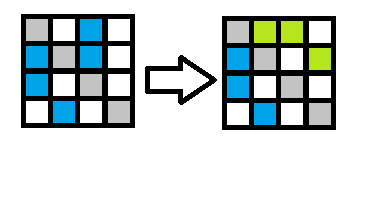
\includegraphics[scale=0.6]{Figures/flip_matrix}
\caption{How the adjacency matrix is flipped on the diagonal}
\label{fig:flipDiagonal}
\end{figure}
\chapter{Related Work}  \label{relatedWork}


In this chapter, we will look at the state of research regarding High-Level Synthesis, information diffusion, and optimization of independent cascade model and breadth-first search.

\section{Information Diffusion} 
There are multiple studies done regarding information diffusion. Studies show how information diffusion can be applied during an disease outbreak\cite{InformationDiffusionThroughBlogspace}, viral marketing\cite{ViralMarketing}, coordinat during crisis situation\cite{Starbird:2012:RRI:2145204.2145212}. 

Different models of information diffusion have been done on blogs\citep{Adar:2005:TIE:1092358.1092473}\cite{GomezRodriguez:2010:IND:1835804.1835933}, and Twitter\cite{Bakshy:2011:EIQ:1935826.1935845}. We can see that in an age of social media, the studies of information diffusion is more relevant than ever. 

While \cite{InfoDiffAndExternalInfluInNetworks} have argued that the emerging of social networks and media have changed the traditional model. The activation is no longer only relying on neighbour vertices, but also an external influence. They found that a large amount of information volume in Twitter is the result of network diffusion, while a small amount is due to external events and factors outside the network\citep{InfoDiffAndExternalInfluInNetworks}. Another study shows that during the 2011 Egyptian Uprising, how a large amount of rebel movement were "tweeted"\cite{Starbird:2012:RRI:2145204.2145212} during the uprising.

As we mentioned in Chapter \ref{background}, we mainly focus on two common information diffusion models, ICM, and LTM. But there are different models too. \cite{5694014} proposed several different problems with traditional models where each vertex is either \textit{activated}(infected, influenced, '1') or \textit{inactive}(healthy, not reached, '0'), and passes the \textit{contagion}(information, data, infection, influence) to neighbouring vertices through the edges. The report mentioned different assumptions that such models make. Among them is that a complete graph is provided, the spread of contagion is from a known source, and that the structure of the network is sufficient to explain the behaviour\citep{5694014}. The report proposes an alternative model, \textit{Linear Influence Model}(LIM), where the focus is on the global influence that an infected vertex has on the rate of diffusion through the implicit network. This model makes the assumption that newly activated vertices are dependent on previously activated vertices. The LIM does not need explicit knowledge of the entire network. Instead, the model takes the newly activated vertices and models them as a \textit{influence function}, which is used to find the global influence.     

\section{High-Level Synthesis}
High-Level Synthesis as a concept has been around since the mid-1980s and early-1990s\cite{HLSTutorial}\citep{HLSPastFutur}. Carnegie-Mellon University design automation (CMU-DA)\citep{1085036}\citep{Parker:1979:CDA:800292.811694} was a pioneering early version of HLS tools. The tool gathers quickly considerable interest. Many HLS tools were built in later years mostly for prototyping and research\cite{Granacki:1985:AAD:317825.317970}\citep{Paulin:1986:HMA:318013.318055}\citep{4069894}. Some of these were able to produce real chips, but the reason for the lack of further development and adaptation was that RTL synthesis was not a widely accepted and an immature field. This often lead to suboptimal solutions. 

Around the year 2000, new HLS tools were developed in academia and the industry. These tools, used high-level language, C and C++. Vivado HLS, designed by Xilinx \citep{6409453}, is one such HLS tool. The Vivado HLS became free during their 2015.4 update\citep{VIVADOHLS}. This resulted in a revived interest in HLS. The community around HLS is also evolving, on the Xilinx-forum, there are multiple answers and active members. We can see that the solution designed by HLS tools is close to traditional hand-crafted designs\citep{6718388}.

Cong et al,\cite{HLSTutorial} discusses different problems and reason for failed commercialization of early HLS tools.  concluded that the problem with the early HLS tools can be summarized by the following reasons: "Lack of comprehensive design language support", "Lack of reusable and portable design specification", "Narrow focus on datapath synthesis", "lack satisfactory QoR", and "Lack of a compelling Reason/event to adopt new design methodology".

 Early versions of HLS tools was not a C-to-RTL transformation. Most of them needed a custom \textit{Hardware Descriptive Language}(HDL). Lacking reusable and portable design specification resulted in that HLS tools required users to include detailed information regarding timing and interface information into source codes. This resulted in a target dependent solution and can't easily port to other devices. The narrow focus on datapath synthesis resulted in a lack of focus on an interface to other hardware modules and platform integration. Those aspects were left to the users to solve system integration problem. The lack of foundation to accurately measure HLS result and often failed to meet timing and power requirement with early HLS tools were another limiting factor. The last reason was that there was no real driving force to turn developers over to such a young and early development format. HLS tools showed exciting capabilities, but most developers did not want to move from the safe and tested RTL design methodology. The paper concludes with that current(2011)HLS tools showed tremendous potentials in becoming standard in selected deployment.

\subsection{Applications using HLS}
In \citep{Malazgirt:2015:HLS:2889287.2889299}, HLS was used to design an accelerator for database analytic and SQL operation. The design was implemented on a Virtex-7 xc7vx690t-g1761-2 FPGA with a focus on accelerating operations; join, data filter, sort, merge and string matching. The accelerator was implemented in C++ in Vivado HLS and optimized with UNROLL directive, PIPELINE directive, and ARRAY\_PARTITION. The UNROLL directive unroll all of the specified loops, while the PIPELINE directive allows multiple accelerators to process data at each clock cycle. The ARRAY\_PARTITION directive partition data into registers.  The accelerator showed promises, giving a 15-140$\times$ speedup compared to Postgres software DBMS running selected TPC\-H queries. 

\cite{Bailey:2015:ALH:2789116.2789145} explored the advantages and disadvantages of HLS implementation of image processing. They argued that custom algorithms on FPGA platforms will most likely result in an improvement, but the algorithms must be tailored to the platforms. The author conducted different case studies to show both the strengths and the weaknesses of HLS. The report goes through image filtering, connected component analysis and two-dimensional fast-Fourier transformation(FFT). One example that the author brings up is during image filtering where HLS was not able to identify the standard accessing pattern during special cases. This resulted in that the HLS built additional hardware to counter such an exception. The report concluded that while HLS can significantly reduce development time and improve utilization of the design space, it is still important to focus on careful design.  The report concludes that HLS can offer many benefits, and is an improvement over conventional RTL-designs, but is not a replacement for hardware designers or clever designs. 

\cite{Butt:2016:DPH:2888407.2871737} implemented a fast Fourier transform (FFT) algorithm for different digital system processing application in HLS. There the authors used Simulink for verification of their design, and implemented it in HLS.

\cite{Zuo:2013:IHL:2435264.2435271} discuss improvements to the current HLS tools with polyhedral transformation. Here they present a problem with HLS, which is that unless the code is inherently compatible, HLS can not apply most of the optimizations. Zuo et al. proposed the polyhedral model, the model takes data dependent multi-block program as input and performs three steps: Classification of array access patterns, performance Metric, and implementation. During the classification of array access patterns, a set of data access pattern is defined and classified. Then the appropriate loop transformation is applied. The next step, the performance of each loop transformation with data-dependency is estimated, and the best improvement is chosen. In the final step, the chosen solution, loop transformation, and inserting HLS directive are applied. Then an interface block for the data-dependent blocks is generated. The generated communication block is then optimized depending on how it behaves. The paper concludes with that the polyhedral model can model can find important loop transformation, thus enable optimization such as pipeline and parallelization.

\cite{6718388} is a case-study where HLS is used to implement two compute heavy machine learning techniques with different computational properties. The two algorithms that were tested was \textit{Lloyd's Algorithm} and a \textit{Filtering Algorithm}. The result was that for the first case, a similar performance between the HLS solution and a hand-written solution, while the second algorithm was severely worse with HLS if the developer did not customize for HLS.
 
\section{Different optimization scheme}
There are a large amount of different optimization research on graph traversal, especially on Breadth First Search. 

\citep{HybridBFS2015} proposed a hybrid FPGA-CPU heterogeneous platform for BFS. The idea is to run the first couple of steps on the CPU core, then switch over to the FPGA accelerator to explore the rest of the graph. The CPU is better suited for calculating while there is a smaller frontier, while the FPGA core is better suited for a larger frontier. By exploiting the characteristics of small-world networks where the frontier is much larger after two-three iterations, one can significantly improve computation time. The report proposed an alternative method of performing the breadth-first search. By performing it as a sparse matrix-vector multiplication over a boolean semiring, more parallelization option was discovered. The result was a speedup of 7.8 compared to a pure software implementation ,and 2$\times$ better compared to an accelerator-only implementation. 
 
\citep{beamer2013direction} propose a hybrid solution, combining a conventional top-down algorithm and a novel bottom-up algorithm. The optimization in this paper focuses on examining fewer edges, thus reduce computation time and trying to circumvent one major drawback with BFS; memory-bound on shared memory. The top-down approach is the traditional algorithm, where a frontier expands and visits all vertices on that level, before each vertex checks its neighbour for unvisited vertices. Unvisited vertices are placed in the frontier vector and marked as visited. The bottom-up algorithm, contrary to the top -down the algorithm, is where each children vertex tries to find a potential parent. A neighbour vertex can be the parent if the neighbour is also in the frontier vector. This results in that after a vertex finds its parent, there is no need to traverse the rest of the frontier. By using different approach during different time, the report was able to achieve a speedup of 3.3 - 7.8$\times$ on synthetic graphs and 2.4 – 4.6$\times$ on real social network graphs.
\chapter{Design and Implementation} \label{methode}
In this chapter, we will present our implementation of the sparse matrix vector multiplication (SpMV) over boolean semiring, how we implemented with HLS and how we connected the IP-cores in the FPGA.

\section{IP-core}
For this project, we have implemented an IP-core with Vivado HLS. The IP-core applies a modified version of SpMV over a adjacency matrix and a set of vertices known as seed nodes. We will givee a brief introduction to HLS programming and how to customize the algorithm for HLS.

\subsection{IP-core}
Our implementation of the SpMV is done in HLS. The algorithm takes in an adjacency matrix and a set of seed nodes as input, and outputs a result vector showing which nodes were activated. The algorithm stops when all the nodes have been activated or it is unable to find any new candidates. Unlike normal SpMV, where each iteration will activate all their neighbours, an ICM is dependent on random number generator (RNG) and a global or local probability. For this project a global probability of 5\% was used, i.e. each node had a 5\% chance of being activated. If $v_1$ was not activated by $V_r$ on the first iteration, $V_r$ can not reactivate $v_1$ on the next iteration. To prevent a reactivation, as mentioned above, a frontier vector will be sent in instead of the result from previous iteration. 

A vector is a list of vertices. The frontier vector is generated by comparing the result from current iteration with a list of activated vertices. The vertices that are in the frontier are the vertices that were not activated in the previous iteration, but were activated in current iteration. 

Our algorithm applies SpMV over the matrix and the frontier. For each iteration, each element in a row of the matrix is applied an AND (\&\&) operation with the corresponding element in the frontier vector. The results from these operations will be ORed ($\|$) together, which gives the result for the row.:
\begin{algorithm}
\begin{algorithmic}[2]
\State{(martix\_row[0] \&\& frontier[0])$\|$(matrix\_row[1] \&\& frontier[1])$\| \ldots$\\
(matrix\_row[n] \&\& frontier[n])$=$result[row]}
\end{algorithmic}
\end{algorithm}


Unlike the breadth first search on boolean semiring, each node will have a chance to not be activated (set as '1'), even if matrix\_row[x] and frontier[x] = 1. This resulted in that for each \&\&- operation, we need to \&\& another \textit{coin toss}, which determined if the activation takes place. The coin-toss is determined by the RNG and the global probability. 

The algorithm will continue until either all of the vertices are activated, or no more vertices can be activated. This is solved with the dist\_gen() function as we mention [INSERT PSEUDOCODE]. The function stops the algorithm when either no more vertices are activated in frontier vector, or all the vertices in the result vector is activated. 

In the high level impleme the implementation of the the algorithm was done in two levels. The top level was the \textit{TopLevelWrapper}. The TopLevelWrapper was set as the main function in our HLS implementation. The function takes in the address of the location of the matrix, the address of the result, and the address to the frontier. Since we are working with ICM, a global probability, a random seed as the initial state for the LFSR is also set as input. The  TopLevelWrapper stores the useful data in a local buffer, where it is sent to the datapth-function. The datapath-function is a sparse martix vector multiplication. 

The address to matrix, result,frontier, and the random seed and global probability is all mapped as AXI4-Lite while the matrix, frontier and the result are memory mapped. This allows us to send in the address of the memory location where the variables are stored and apply our algorithm. 
 
Since ICM is dependent on a random function, we ran each sets of seed nodes 50 times to find the average runtime and coverage to find the most optimal set of nodes.

\section{Linear-Feedback Shift Register}
The LFSR is a commonly used pseudorandom number generator(pRNG)\citep{murase1992linear}. Different sized LFRS is able to generate a wider range of pseudo random numbers. LFSR generates a pseudorandom number based on the previous pseudorandom number it generated. The LFSR implemented for this project is a 16 bit shift register, that is able to generate a pseudorandom number in the range from 0-$2^{16}(65536)$. In order to generate the new number, the bits from positions 16,14,13 and 11, is XORed. I.e. (((16 XOR 14) XOR 13 ) XOR 11) = new bit. The new bit is pushed into bit-position 1 and the entire registers shifts towards right 1 bit. 
This allows the IP-core to generate a pseudorandom number based on a initial seed input. From Figure: \ref{fig:LFSR} we can see that to continuously generate pseudo random numbers the output from the LFSR is used as the next iterations seed. 

\begin{figure} 
\includegraphics[scale=0.5]{Figures/LFSR}
\caption{16-bit Linear-Feedback Shift Register}
	\label{fig:LFSR}
\end{figure}


\section{Design flow of HLS}
For this project, Xilinx Vivado HLS 2016.1 was used. The usual workflow in designing with Vivado HLS is as follow. 
\begin{enumerate}
\item Define your funciton/algorithm.
\item Simulate as compile code. 
\item Synthesise.
\item Co-simulate.
\end{enumerate}

There are some steps that Vivado HLS requires before the project can start. In the begining, Vivado HLS would require the designer to specify which function is the top level of the implementation. That top function would determine which port the IP core would have and what type of AXI4 protocol to implement. Vivado HLS also enables the user to specify to which platform this implementation is for.


The first step in designing with Vivado HLS is to define the algorithm that will be synthesised. E.g. for this report, its the matrix vector multiplication. After identifying different requirements and dependencies, the algorithm is implemented in C with Vivado HLS. Vivado HLS has some limitation regarding the high level implementations:
\begin{itemize}
\item No dynamic memory (Need to be static), Vivado HLS does not support malloc, free, new or delete. 
\item NO STD, FILE-IO, etc, (no system calls). 
\item avoid recursive functions. 
\end{itemize}

The next step is to \textit{run C simulation}. This will verify that the C implementation is correct, by running the test in the testbench. The test in the testbench are created by the designer. After verifying that the implementation is correct, next step is to synthesise the implementation. Vivado HLS will then generate the appropriate Verilog or VHDL, depending on  the designer choice. The finished generated solution is then reviewed by reading the Vivado synthesise report. The report containing crucial information regarding the generated solution. There we can find the performance estimates of the generated core, the utilization estimates, and the interface to the generated core. After all this is done, Vivado offers a \textit{run C/RTL Cosimulation}. Vivado will then run both the C simulation and testbench, and the same testbench on a simulated version of the implemented core. This function allows the designer to verify that the generated core have the same behaviour as the simulated C implementation.

After Cosimulation is done, the IP-core is ready for export. \textit{Export RTL} generates the necessary RTL files and exports the IP core. The exported IP-core can then be found in the project folder and is ready to be uploaded to the FPGA. 

The input and output port of the IP core is determined by the variables that the top function require. variables that are read from, will automatically be set as input, while variable that are only written to, will be set as output. In order for the core to understand what is mutable, the output is often set as a pointer (For C code). VIVADO HLS generates control signals cl automatically. 

\section{Network and graph generator}

For this project, we choose to implement a R-mat generator as mentioned in Chapter: \ref{rmat} and  \cite{Rmat2004}. The generator is implemented in \textit{Python} \cite{PYTHON} with \textit{numpy}. The generator generates adjacency matrix with $2^k$ nodes, where \textit{k} is known as the scale of the sparse matrix. The total amount of edges the graph contains is set as $total\_amount\_of\_edge = k \times\ edge\_factor $. The edge factor is the ratio between the graph's edge count and ins vertex count\cite{graph500}.



\section{How is it connected}
As shown in Figure \ref{fig:vivadoImple}, out IP-core is the \textit{TopLevelWrapper}, and the PS is the Zynq processing system. The AXI interconnect serves as a interconnect between our IP-core and the PS.

\begin{figure}[!ht]
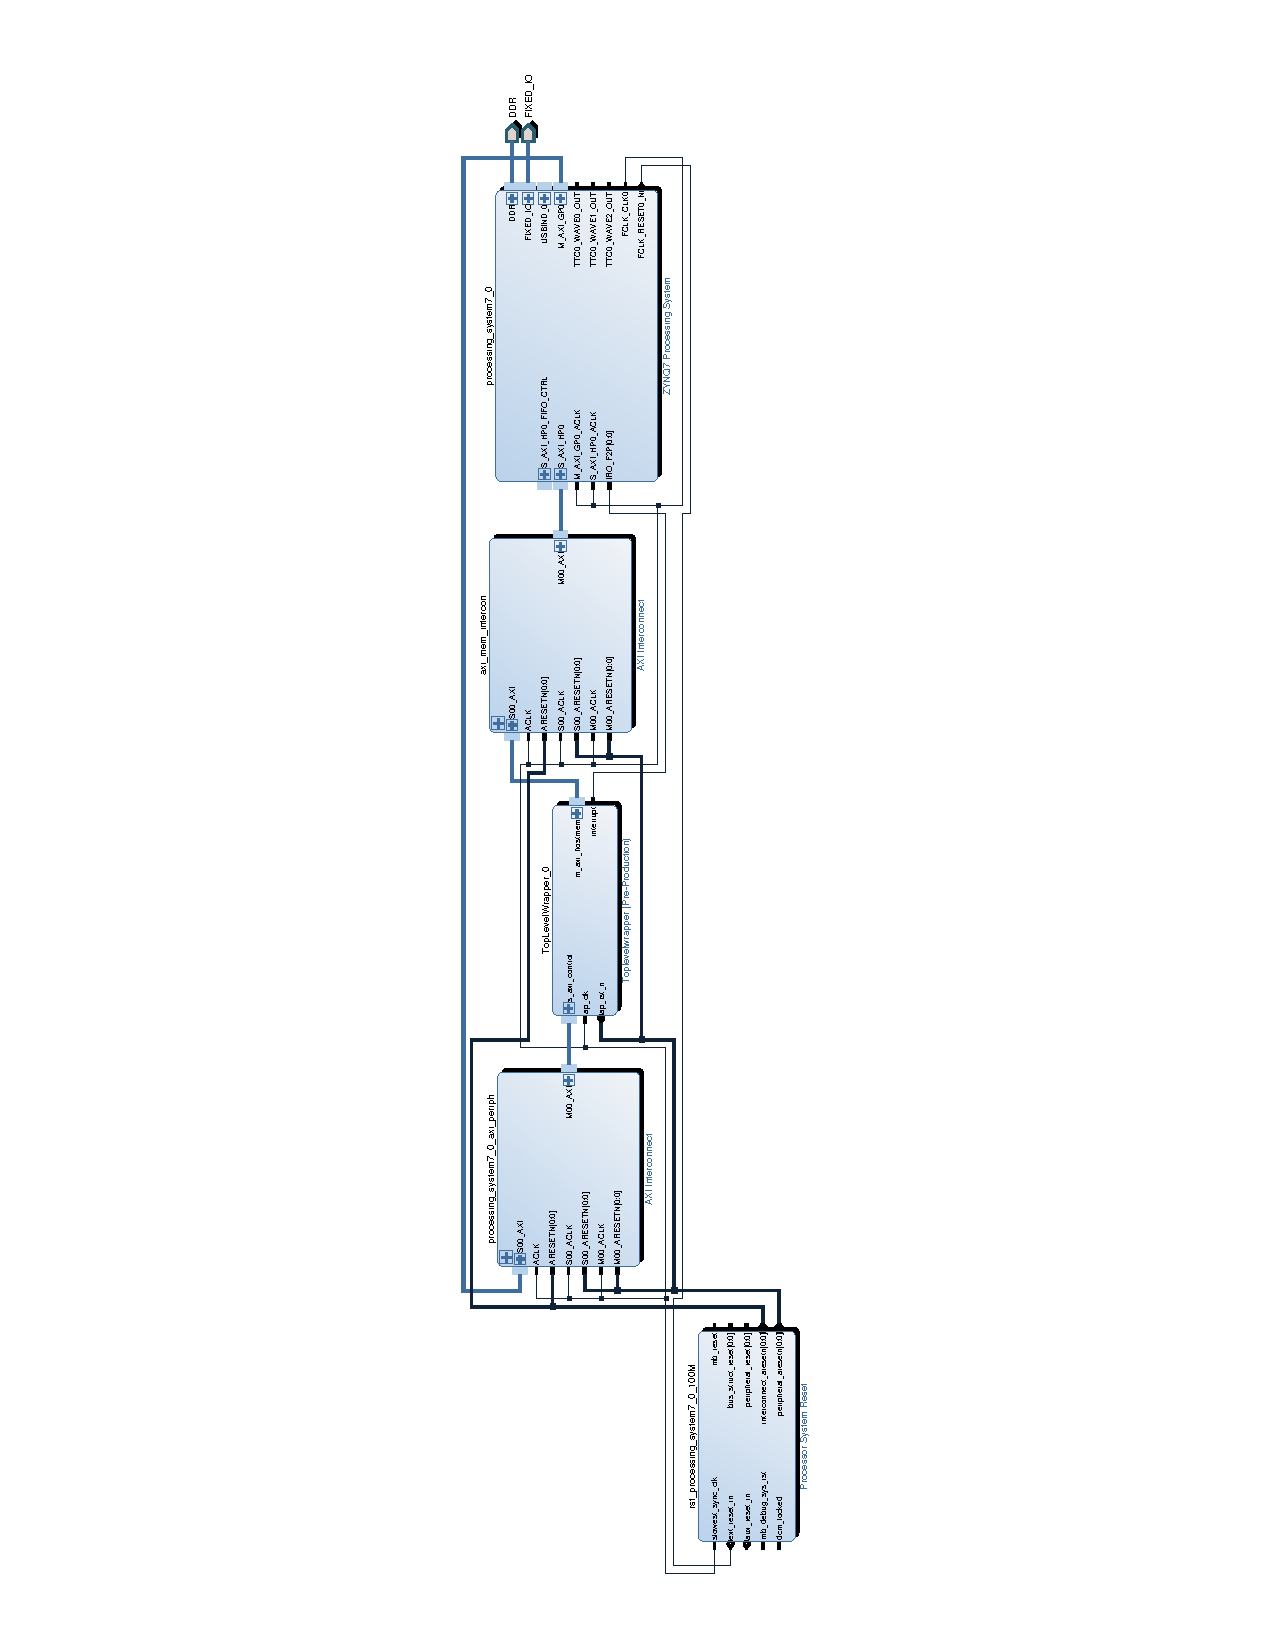
\includegraphics[scale=0.7]{Figures/design_1}
\caption{Our IP-core and how it is connected.}
\label{fig:vivadoImple}
\end{figure}



Our core is memory mapped and we se the bus interface AXI4-Lite for communication. The core includes an dma-component, which the HLS would initiate for us. This allows us to utilize the High performance slave interface on our PS.


\section{Xilinx SDK}
Vivado offers a \textit{Eclipse} based software develop kit (SDK). There we read the pregenerated graph from a SD card on the ZedBoard. We initiated the the custom IP core by setting all the required input signals.

%Snakk litt om hvordan din seed search er implementert via xilinx sdk%



\section{Optimization}
The function matrix\_vector\_multiplication() performes a single matrix vector multiplication. From the pseudocode, we can see that there is a room for parallization of the SpMV. The outer for loop from the pseudocode, can be parlized since the for loop is not dependent on the variables from the inner for-loop. 

Another possible paralization is during the simulation, after the spmv, the frontier needs to be calculated. And a converged() function is called in the end to determen if the simulation is finished. The frontier calculation and converged can pe run in parallel. 

include the different directives, PIPLINE

THe IP-core (currently) is only using around 2\% of the resource available on the FPGA(Zedboard). This gives us a lot of room for parallization of different core. Implemented 2 bus, one for input stream, one for output stream. The output stream consist of the result\_vector




\section{Potential improvement}:
For the second option, where the RNG core is not implemented into the IP CORE, we would have to have teh random number set as AXI4 stream from the buffer, since we would need to call a stream of random number from the core.


\section{global vs local probability}
For this project, a global activation chance was implemented, giving each node the same probability to be activated. A interesting model would be there are a personal probability of activation. Each node might have unique activation chance. Our implementation. 

\chapter{Result and Discussion} \label{result}

as we can see, the algorithm was able to finish a extreme scaled down version of the original sparse matrix. This is unfortunate, since our goal was to iterate over large graphs. But these results are still interesting and proves that HLS can be an improvement.
We were able to run a implementation with pipeline and loop unrolling, but that resulted in a too large core and the synthesiser took over 24 hour to synthesise, Which was too long and was therefore abandoned.
This resulted in that most of the numbers here are taken from Vivado HLS simulation and Cosimulation. |

\section{•}

\section{Performance}
As we can see, the hardware implementation is better then the C-simulated implementation, even at this low scale, we can see that the

We have here included a snapshot of our synthesis report. As we can see, we have a rather large utilization of look up table(LUT) and flip flop(FF). This is the result of the PIPELINE and Loop unrolling. Our high level implementation does contains several Loops and dependencies, this results in a large amount of resource used. 

We used the following variables to generate our adjacency matrix:
\begin{itemize}
\item \textbf{A} = 0.57
\item \textbf{B} = 0.19
\item \textbf{C} = 0.19
\item \textbf{D} = 1-0.57-0.19-0.19 = 0.05
\item \textbf{Edge factor}  = 16
\item \textbf{k (Scale)} = 4
\end{itemize}

By using the random-function provided by Python, we placed '1' in it's correct place. After the matrix is generated, we further applied a diagonal copying as shown in Figure:\ref{fig:flipDiagonal}. This is obligatory to generate an undirected graph.

For this project, a graph with size 1024 was used. This is a microscopic graph compared to graphs used in network analysis. 

\begin{figure}
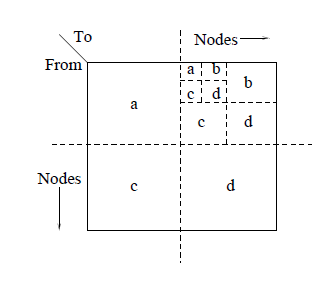
\includegraphics{Figures/Rmat}
\caption{The R-mat model \cite{Rmat2004}}
\label{fig:Rmat}
\end{figure}



\section{Discussion}
\subsection*{Analysis of the performance}
Our IP core was originally designed for networks with 1024 vertices, but after implementing with the optimization directives, the resource usage were out of bound. This resulted in a severe scale down for this project. The resulted network was down to the size of 16 vertices. In network analysis, this is such a small scale that the results from this experiment would only serve as a proof of concepts. 
 
\subsection*{problem that was encountered}
One problem that was encountered during this project was that the output signal from the synthesiser was not the correct direction. The output signal was often set as input signal. The HLS would automatically set the values as output signal or input signal.The reurn value from a funciton would be set as a the output signal, while the variable that the function takes, would be set as the input signal. Another way wo specify that something is the output signal would be to explicitly set them as pointer arguments. This will in set the signal to be output signal.

Another problem that I often encountered, was that the Vivado HLS often stop working. The problem was fixed by creating a new project and include the previous files.

Another problem, was that some times the Vivado HLS was not able to Cosimulate the implementation the first time. I was not able to find a solution to this problem except resynthesis the project. 

There were incidence where the implementation on the Zedboard did not behave as the implementation. This was solved by reprogramming the device and sometimes, restarting the Zedboard.


\chapter{Future work} \label{futureWork}
Information diffusion and seed selection in general computes gigantic graphs, and thus is very time consuming. There is therefore several performance related improvements that have yet to be explored.

\begin{enumerate}
\item \textbf{Different architecture} for this implementation, we used a core including the LFSR, it would be interesting to explore different architecture. One solution that we did not have the chance to explore, is implement a large buffer connected to a single LFSR that continuously generates random number. The implemented cores would then each pop one random number for each cointoss. This solution requires a large buffer and would potentially generate large overhead with reading from the buffer. A large enough buffer  would also be required since there are in worst case scenario for a single SpMV run, we would need $n^2$ cointoss. The potentially benefits of such a design would be better space utilization. A smaller core would use less resource of the Zedboard. This can result in more parallelization.

\item \textbf{Use larger graph} In graph theory, graph used is often at scale(26-42). The smallest mentioned graph from Graph500, is $2^26$, a toy graph. Our graph is not even close to such a large graph.

\item \textbf{Customize algorithm} As mentioned in Chapter \ref{relatedWork}, HLS can generate a close to hand written design if the algorithm is customized for HLS. A interesting potential improvement would be to analyse algorithm and explore different solutions and implementation.

\item \textbf{Compare different solutions} In this report, we have only showed the result from one architecture, it would be interesting to compare different shcems

\item \textbf{Memory Optimization}. For this algorithm, we store the entire adacency matrix. This is inefficient for a sparse matrix. An potentially improvement would be to explore a different storage format for the adjacency matrix.

\item \textbf{Try different seed selection algorithm}
\end{enumerate}


The community of the HLS is very active and frequently responds to forum post seeking help.	Not many work that uses HLS[CITATION NEEDED]. Recently was free, used to cost money.


Learn more about HLS so it can be better utilized. 
different scheme to further work:
- implement parallel
- different scheeme, rng on the outside
- Use other data structure.
- larger graph
- compare this solution to other solution, 
- implement more efficient memory storage
- use other storage method since its sparse. 
- would be interesting to gather information on  energy consumption.
- Implement a more general architecture to handle more total vertices.
- If  there would be enough memory on the board, would be interesting to run 50 times on the board and just return the avrage time and coverage

\chapter{Conclusion}
In this report, we have explored the possibility to use HLS as an implementation tool to accelerate seed selection for information diffusion. We used a modified version of sparse matrix-vector multiplication to perform ICM iterations. We have implemented a simple IP-core that applies ICM with an adjacency matrix and a set of seed nodes. The core returns the percentage of infected nodes in the network. The design was loaded onto an FPGA and multiple tests were conducted both on the chip and in the simulation.

In this project, we were not able to synthesise an IP-core that could compute large matrices. By synthesising an  IP-core with s larger buffer, the resource usage was much higher than what was available on our Zedboard. This is likely the result of lack of customization of the high-level implementation.
 

\textbf{Task 1 \textit{(mandatory)}} Implement information diffusion as sparse matrix-vector multiplication, with high level language C. Completed
\\

W have in this project implemented a modified sparse matrix-vector multiplication that perform ICM. The implementation detail can be found in Chapter \ref{methode}, and the theory can be found at \ref{background}  \\ \hfil \\ \hfil
\textbf{Task 2 \textit{(mandatory)}} Tailor the implementation of Information Diffusion for synthesise with Vivado HLS. Complete \\

The design was able to synthesise in Xilinx Vivado HLS and gave back somewhat interesting results. The detail about the HLS and different optimization used can be found at chapter \ref{methode}.  \\ \hfil \\ \hfil
\textbf{Task 3 \textit{(optional)}} Implement said design on a  Zynq FPGA board.\\

Out IP-core was able to upload on the FPGA and gave back the result. Chapter \ref{result} presents the result from the FPGA and other 
 \\ \hfil \\ \hfil
 
\textbf{Task 4 \textit{(optional)}} Extend the system to be able to handle graph in the size of toy graphs(containing $2^{26})$ vertices) \\ \hfil \\ \hfil

Due to unfamiliarity with HLS and time constraints. We were not able to extend the system to compute larger graph.  \\



\bibliographystyle{unsrt}
\bibliography{my_references}
%\bibliography{website_references.bib}


\end{document}     